\section{Lee Model}

\begin{frame} {Lee Model}
    \begin{itemize}
        \item Three phases: break down, axial, and compression phases.
        \item Compression phase: inward shockwave, reflected shockwave, and slow compression phase.
    \end{itemize}
\end{frame}

\begin{frame} {Break Down Phase}
    \begin{itemize}
        \item Gas is ionized, and current layer formed
    \end{itemize}
    \begin{figure}
        \centering
        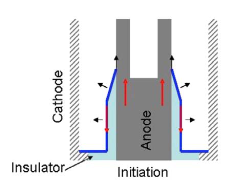
\includegraphics[width=0.5\textwidth]{figures/breakdown-phase.png}
        \caption{Initiation via flashover of the insulator. Break down phase. \cite{krishnan_2012_dense}}
        \label{fig:breakdown-phase}
    \end{figure}
\end{frame}

\begin{frame} {Axial Phase}
    \begin{itemize}
        \item Current layer is accelerated by the $\mathbf{J\times B}$ force in the axial direction.
        \item A shockwave (SW) is formed due to magnetic pressure (MP).
    \end{itemize}
    \begin{figure}
        \centering
        \begin{subfigure}{0.5\textwidth}
            \centering
            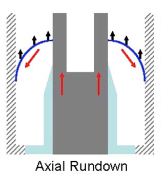
\includegraphics[width=0.5\textwidth]{figures/axial-rundown.png}
            \caption{Axial run-down phase. \cite{krishnan_2012_dense}}
        \end{subfigure}%
        \begin{subfigure}{0.5\textwidth}
            \centering
            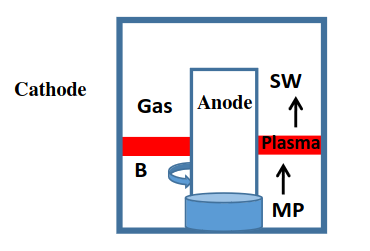
\includegraphics[width=0.7\textwidth]{figures/axial-phase.png}
            \caption{The formation of plasma layer. \cite{behbahani_2017_enhancement}}
        \end{subfigure}
        \label{fig:axial-phase}
    \end{figure}
\end{frame}

\begin{frame} {Compression Phase - Inward Shockwave Phase}
    \begin{itemize}
        \item When the plasma layer arrives at the top of the anode, the $\mathbf{J\times B}$ force pushes them into the center of the anode.
        \item Plasma column with inner radius $r_s$ and outer radius $r_p$ will form on the top of the anode.
        \item Shockwave compresses gas in the center.
    \end{itemize}
    \begin{figure}
        \centering
        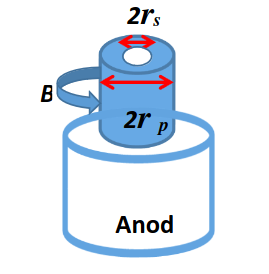
\includegraphics[width=0.4\textwidth]{figures/inward-shockwave-phase.png}
        \caption{The inward radial shock wave in final stage off plasma focus.}
        \label{fig:inward-shockwave-phase}
    \end{figure}
\end{frame}

\begin{frame} {Compression Phase - Reflected Shockwave Phase}
    \begin{itemize}
        \item The shockwave will be reflected radially in the outward direction after hitting the center of the anode.
    \end{itemize}
    \begin{figure}
        \centering
        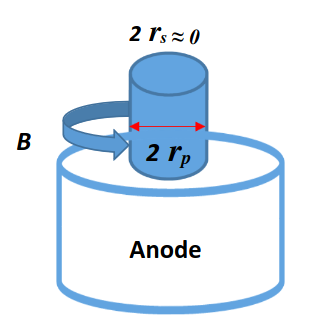
\includegraphics[width=0.4\textwidth]{figures/reflected-shockwave-phase.png}
        \caption{The reflected shockwave phase in plasma focus. \cite{behbahani_2017_enhancement}}
        \label{fig:reflected-shockwave-phase}
    \end{figure}
\end{frame}

\begin{frame} {Compression Phase - Slow Compression Phase}
    \begin{itemize}
        \item Slow compression phase starts when $r_s=r_p$.
        \item The reflected shockwave produces a pressure in the opposite direction of the magnetic pressure.
        \item Plasma column will be compressed to its minimum radius.
    \end{itemize}
\end{frame}

\begin{frame} {Instability Phase}
    \begin{itemize}
        \item When plasma reaches maximum compression, the plasma column may become unstable due to plasma instabilities.
        \item Instabilities make the plasma resistance anomalous.
    \end{itemize}
    \begin{figure}
        \centering
        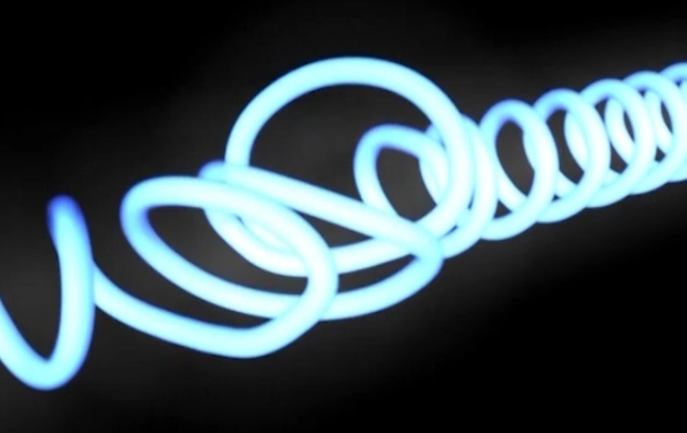
\includegraphics[width=0.7\textwidth]{figures/instability-phase.png}
        \caption{Plasma column is twisted in instability phase. Source \cite{lppfusion_device_fusion}}
        \label{fig:instability-phase}
    \end{figure}
\end{frame}